% act_d6_mp.tex — Iskole: MP / Manager Workflow
\documentclass[a4paper,landscape]{article}
\usepackage[a4paper,landscape,top=1.8cm,bottom=1.2cm,left=1.2cm,right=1.2cm]{geometry}
\usepackage[dvipsnames,svgnames]{xcolor}
\usepackage{tikz}
\usetikzlibrary{shapes.geometric,arrows.meta,calc}
\usepackage{fancyhdr}
\definecolor{ColHdr} {RGB}{30,58,138}
\definecolor{ActFill}{RGB}{219,234,254}
\definecolor{ActLine}{RGB}{52,109,219}
\definecolor{SysFill}{RGB}{220,254,220}
\definecolor{SysLine}{RGB}{34,139,34}
\definecolor{DecFill}{RGB}{254,244,220}
\definecolor{DecLine}{RGB}{204,120,0}
\definecolor{SwimBg} {RGB}{240,240,248}
\tikzset{
  nd_start/.style={circle,fill=black,minimum size=10pt,inner sep=0pt},
  nd_stop/.style={circle,fill=black,draw=black,double,double distance=2pt,minimum size=10pt,inner sep=0pt},
  nd_act/.style={rectangle,rounded corners=3pt,draw=ActLine,fill=ActFill,text width=4.9cm,minimum height=0.62cm,align=center,font=\footnotesize},
  nd_sys/.style={rectangle,rounded corners=3pt,draw=SysLine,fill=SysFill,text width=4.9cm,minimum height=0.62cm,align=center,font=\footnotesize\itshape},
  nd_dec/.style={diamond,aspect=2.4,draw=DecLine,fill=DecFill,text width=2.5cm,align=center,font=\footnotesize,inner sep=1pt},
  arr/.style={-{Stealth[length=5pt,width=4pt]},thick},
  lbl/.style={font=\scriptsize,fill=white,inner sep=1pt},
}
\newcommand{\swimbox}[4]{%
  \fill[SwimBg,rounded corners=4pt](#1-2.6,#2+0.15) rectangle (#1+2.6,#3);
  \node[font=\small\bfseries\color{ColHdr}] at (#1,#2) {#4};}
\pagestyle{fancy}\fancyhf{}
\fancyhead[C]{\bfseries\color{ColHdr}Iskole — Activity Diagram 6: MP / Manager Workflow}
\fancyfoot[C]{\small\thepage}
\renewcommand{\headrulewidth}{1pt}
\renewcommand{\headrule}{\hbox to\headwidth{\color{ColHdr}\leaders\hrule height 1pt\hfill}}
\setlength{\headheight}{16pt}
\begin{document}
\begin{center}
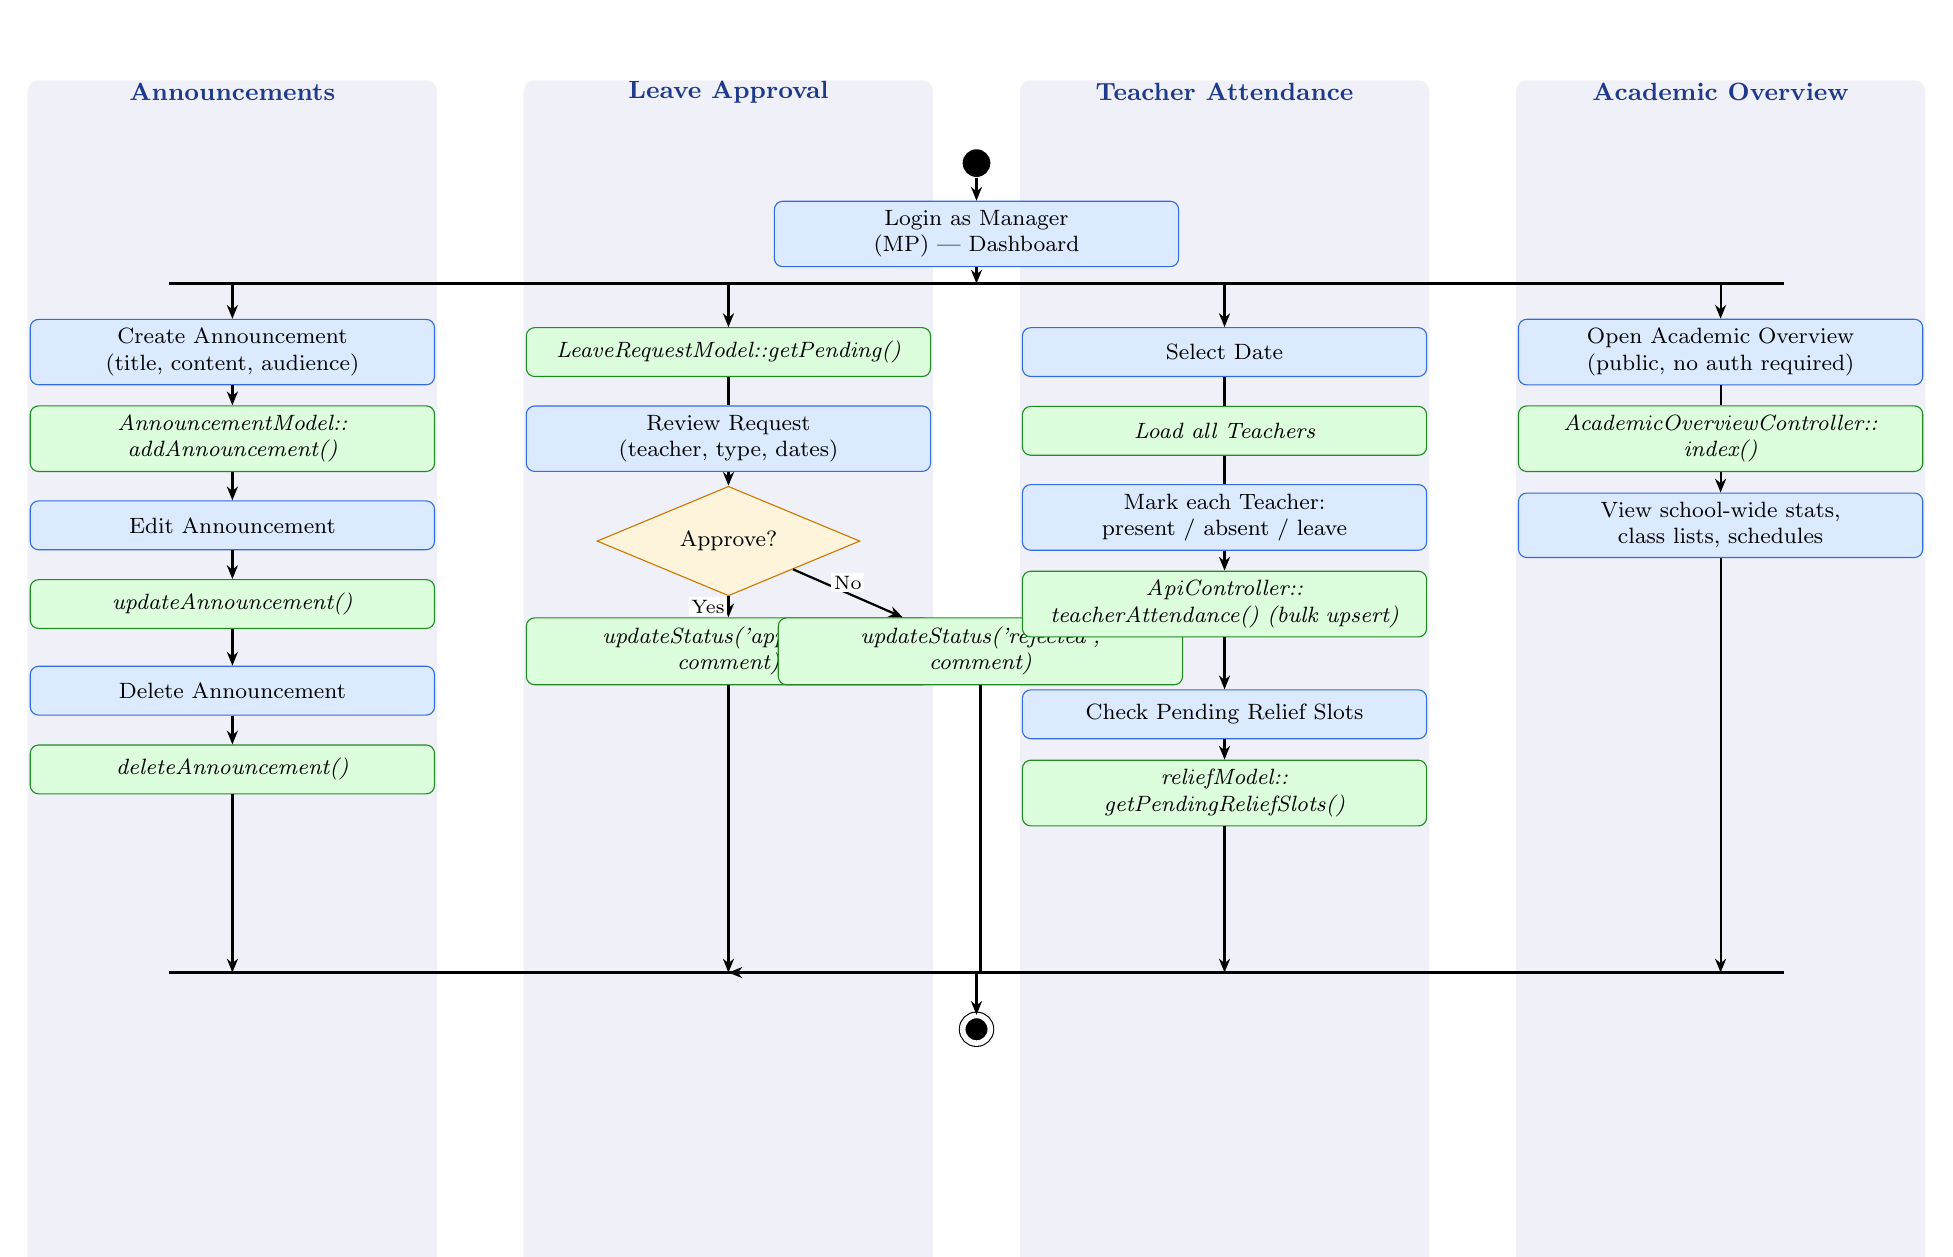
\begin{tikzpicture}[x=1cm,y=1cm]
\def\cA{3.3}\def\cB{9.6}\def\cC{15.9}\def\cD{22.2}
\swimbox{\cA}{0.2}{-14.8}{Announcements}
\swimbox{\cB}{0.2}{-14.8}{Leave Approval}
\swimbox{\cC}{0.2}{-14.8}{Teacher Attendance}
\swimbox{\cD}{0.2}{-14.8}{Academic Overview}
\node[nd_start] at (12.75,-0.7)(S){};
\node[nd_act]   at (12.75,-1.6)(HD){Login as Manager (MP) \textemdash{} Dashboard};
\fill[black](2.5,-2.25) rectangle (23.0,-2.21);
% Col A
\node[nd_act] at (\cA,-3.1)(A1){Create Announcement\\(title, content, audience)};
\node[nd_sys] at (\cA,-4.2)(A2){AnnouncementModel::\\addAnnouncement()};
\node[nd_act] at (\cA,-5.3)(A3){Edit Announcement};
\node[nd_sys] at (\cA,-6.3)(A4){updateAnnouncement()};
\node[nd_act] at (\cA,-7.4)(A5){Delete Announcement};
\node[nd_sys] at (\cA,-8.4)(A6){deleteAnnouncement()};
% Col B
\node[nd_sys] at (\cB,-3.1)(B1){LeaveRequestModel::getPending()};
\node[nd_act] at (\cB,-4.2)(B2){Review Request\\(teacher, type, dates)};
\node[nd_dec] at (\cB,-5.5)(BD){Approve?};
\node[nd_sys] at (\cB,-6.9)(B3){updateStatus('approved',\\comment)};
\node[nd_sys] at (\cB+3.2,-6.9)(B4){updateStatus('rejected',\\comment)};
% Col C
\node[nd_act] at (\cC,-3.1)(C1){Select Date};
\node[nd_sys] at (\cC,-4.1)(C2){Load all Teachers};
\node[nd_act] at (\cC,-5.2)(C3){Mark each Teacher:\\present / absent / leave};
\node[nd_sys] at (\cC,-6.3)(C4){ApiController::\\teacherAttendance() (bulk upsert)};
\node[nd_act] at (\cC,-7.7)(C5){Check Pending Relief Slots};
\node[nd_sys] at (\cC,-8.7)(C6){reliefModel::\\getPendingReliefSlots()};
% Col D
\node[nd_act] at (\cD,-3.1)(D1){Open Academic Overview\\(public, no auth required)};
\node[nd_sys] at (\cD,-4.2)(D2){AcademicOverviewController::\\index()};
\node[nd_act] at (\cD,-5.3)(D3){View school-wide stats,\\class lists, schedules};
% join
\fill[black](2.5,-11.0) rectangle (23.0,-10.96);
\node[nd_stop] at (12.75,-11.7)(E){};
% arrows
\draw[arr](S)--(HD);
\draw[arr](HD.south)--(12.75,-2.23);
\foreach \x/\n in {\cA/A1,\cB/B1,\cC/C1,\cD/D1}{\draw[arr](\x,-2.23)--(\n);}
\draw[arr](A1)--(A2);\draw[arr](A3)--(A4);\draw[arr](A5)--(A6);\draw[arr](A2)--(A3);\draw[arr](A4)--(A5);
\draw[arr](B1)--(B2)--(BD);
\draw[arr](BD)--node[lbl,left]{Yes}(B3);
\draw[arr](BD)--node[lbl,above]{No}(B4);
\draw[arr](C1)--(C2)--(C3)--(C4);\draw[arr](C5)--(C6);\draw[arr](C4)--(C5);
\draw[arr](D1)--(D2)--(D3);
\draw[arr](A6)--(\cA,-10.98);
\draw[arr](B3)--(\cB,-10.98);
\draw[arr](B4.south)--($(B4.south)+(0,-0.3)$)--(\cB+3.2,-10.98)--(\cB,-10.98);
\draw[arr](C6)--(\cC,-10.98);
\draw[arr](D3)--(\cD,-10.98);
\draw[arr](12.75,-10.96)--(E);
\end{tikzpicture}
\end{center}
\end{document}
